% title: Separate rules for one primitive
% description: The same primitive has an abstract rule for tracing, an implementation rule for execution, and separate rules for supported transforms.
% width: 35rem
\documentclass[tikz,border=5pt]{standalone}
\usetikzlibrary{arrows.meta}

\begin{document}
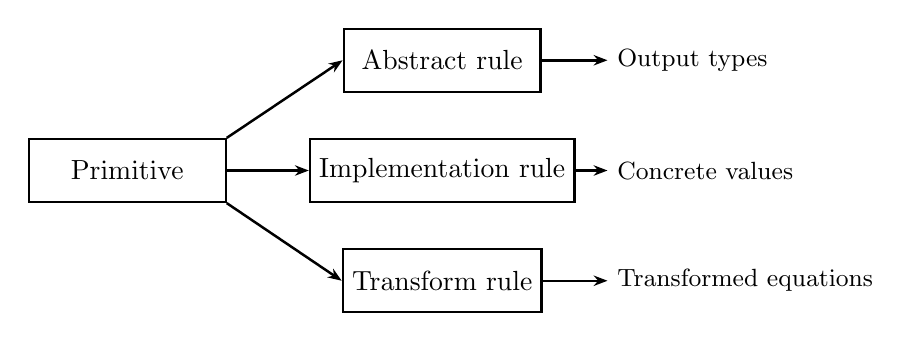
\begin{tikzpicture}[
    box/.style={draw, line width=0.8pt, minimum height=0.8cm,
                minimum width=2.5cm, align=center},
    flow/.style={-{Stealth[length=5pt]}, line width=0.9pt},
    note/.style={font=\small, align=center},
]
    \node[box] (primitive) at (0, 0) {Primitive};
    \node[box] (abstract) at (4, 1.4) {Abstract rule};
    \node[box] (impl) at (4, 0) {Implementation rule};
    \node[box] (transform) at (4, -1.4) {Transform rule};
    \node[anchor=west, note] (types) at (6.1, 1.4) {Output types};
    \node[anchor=west, note] (values) at (6.1, 0) {Concrete values};
    \node[anchor=west, note] (equations) at (6.1, -1.4)
        {Transformed equations};

    \draw[flow] (primitive.north east) -- (abstract.west);
    \draw[flow] (primitive.east) -- (impl.west);
    \draw[flow] (primitive.south east) -- (transform.west);
    \draw[flow] (abstract.east) -- (types.west);
    \draw[flow] (impl.east) -- (values.west);
    \draw[flow] (transform.east) -- (equations.west);
\end{tikzpicture}
\end{document}
